% !TeX spellcheck = en_GB
Besides the efficiency of the networks, the resistance of their predictions to noise is also of interest.
We create a noisy sequence $\{\ket{\phi_n}\}$ of N qubits from $\{\ket{\psi_n}\}$ using
\begin{align*}
	\ket{\phi_n} = e^{-i H_n \tau} \ket{\psi_n} \ \forall n \in [1, N].
\end{align*}
$H_n$ are randomly generated Hermitian matrices with $\norm{H_n} = \sqrt{\Sigma_{ij} \abs{h^n_{ij}}^2} = 1$ and $\tau$ is a real parameter used to control the strength of the noise.
To quantify the dissimilarity between $\{\ket{\phi_n}\}$ and $\{\ket{\psi_n}\}$ we use the fidelity $F$ as defined in \cite{10.5555/1972505}:
\begin{align*}
	F_{\text{run}}(\{\ket{\phi_n}\}, \{\ket{\psi_n}\}) = \prod_n F(\ket{\phi_n}, \ket{\psi_n}) = \prod_n \abs{\bra{\phi_n}\ket{\psi_n}}.
\end{align*}

The performance of the bidirectional LSTM for $\Delta \mathrm{T} = 1$ and $\Delta \mathrm{T} = 5$ on noisy sequences is presented in Figure \ref{noisedt5}.
For $\Delta \mathrm{T} = 1$, the performance degrades among the test set, as the noiseless predictions are near their optima.
The variance in the deviation of work output between noisy and noiseless data $\Delta W = \overline{W}_{noise} - W_{pred}$ is larger for $\Delta \mathrm{T} = 5$ as the longer evolution time leads to a larger difference between the system states of the noisy and noiseless case.
As the network is less likely to predict a solution near the optimum, the noisy data will sometimes be closer to the optimum and thus a significant amount of data points with $\Delta W > 0$ exist as well.

\begin{figure}[h]
	\centering
	\begin{subfigure}{0.4\textwidth}
		\centering
		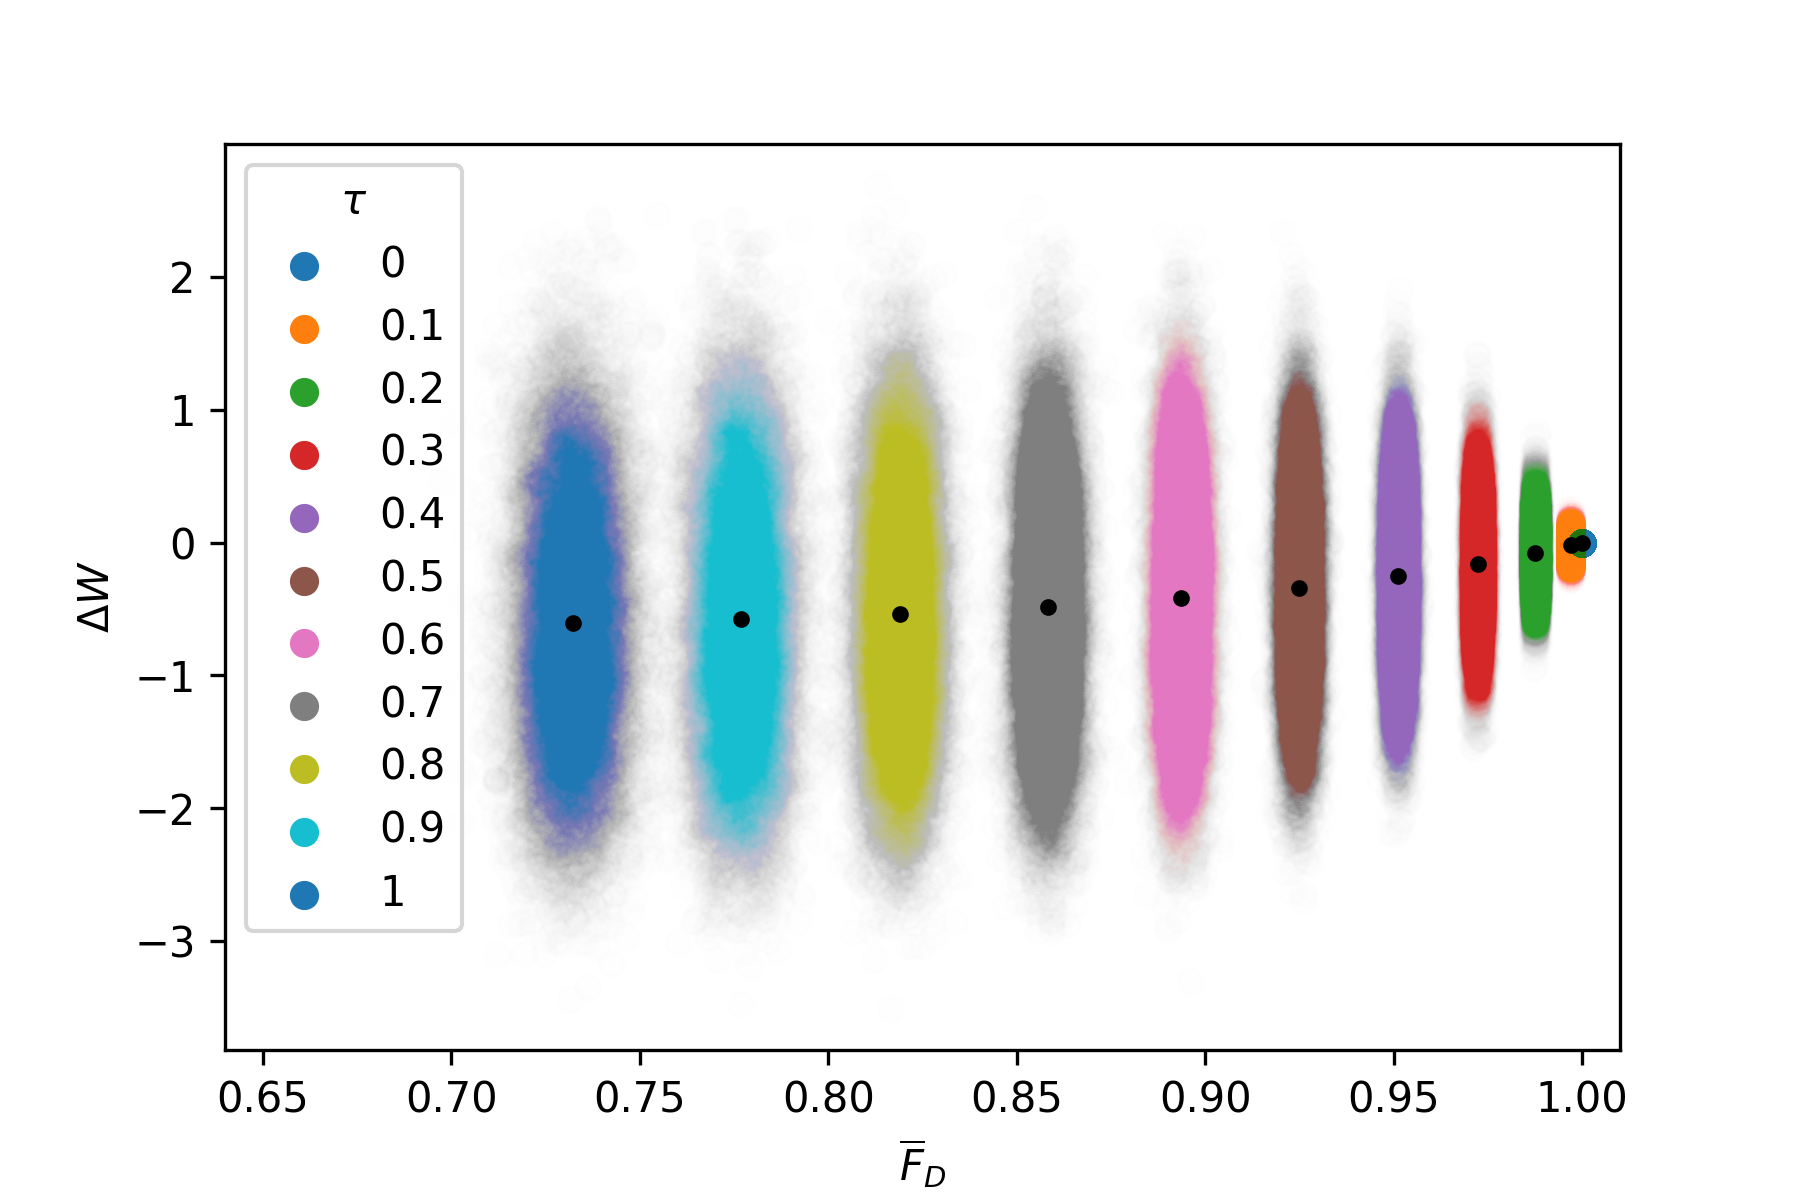
\includegraphics[width=\textwidth]{img/noisy_drive_bi_true_3}
		\subcaption{Noisy drive sequence, $\Delta \mathrm{T} = 5$}
	\end{subfigure}
	\begin{subfigure}{0.4\textwidth}
	\centering
%	Hier kommt noch ein Bild
	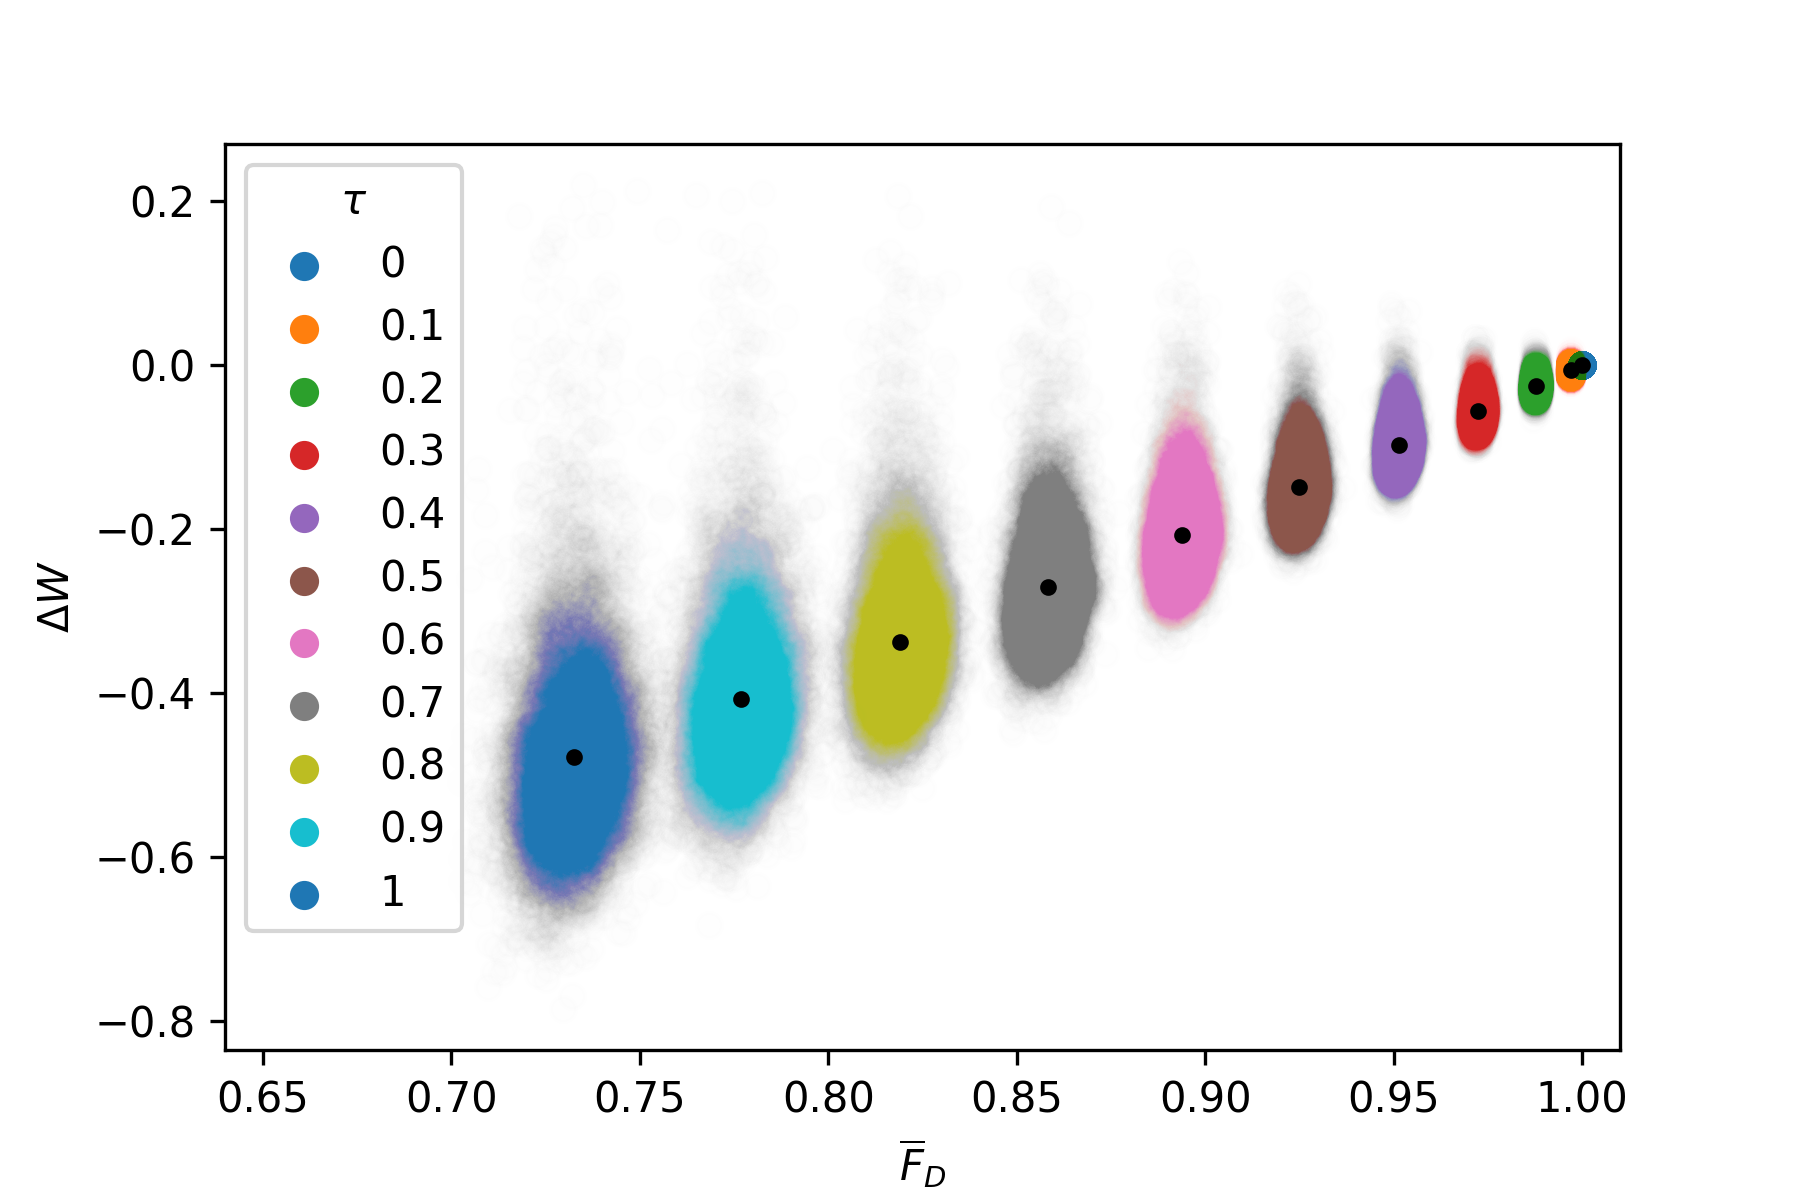
\includegraphics[width=\textwidth]{img/noisy_drive_dt_1}
	\subcaption{Noisy drive sequence, $\Delta \mathrm{T} = 1$}
	\end{subfigure}
	\begin{subfigure}{0.4\textwidth}
		\centering
		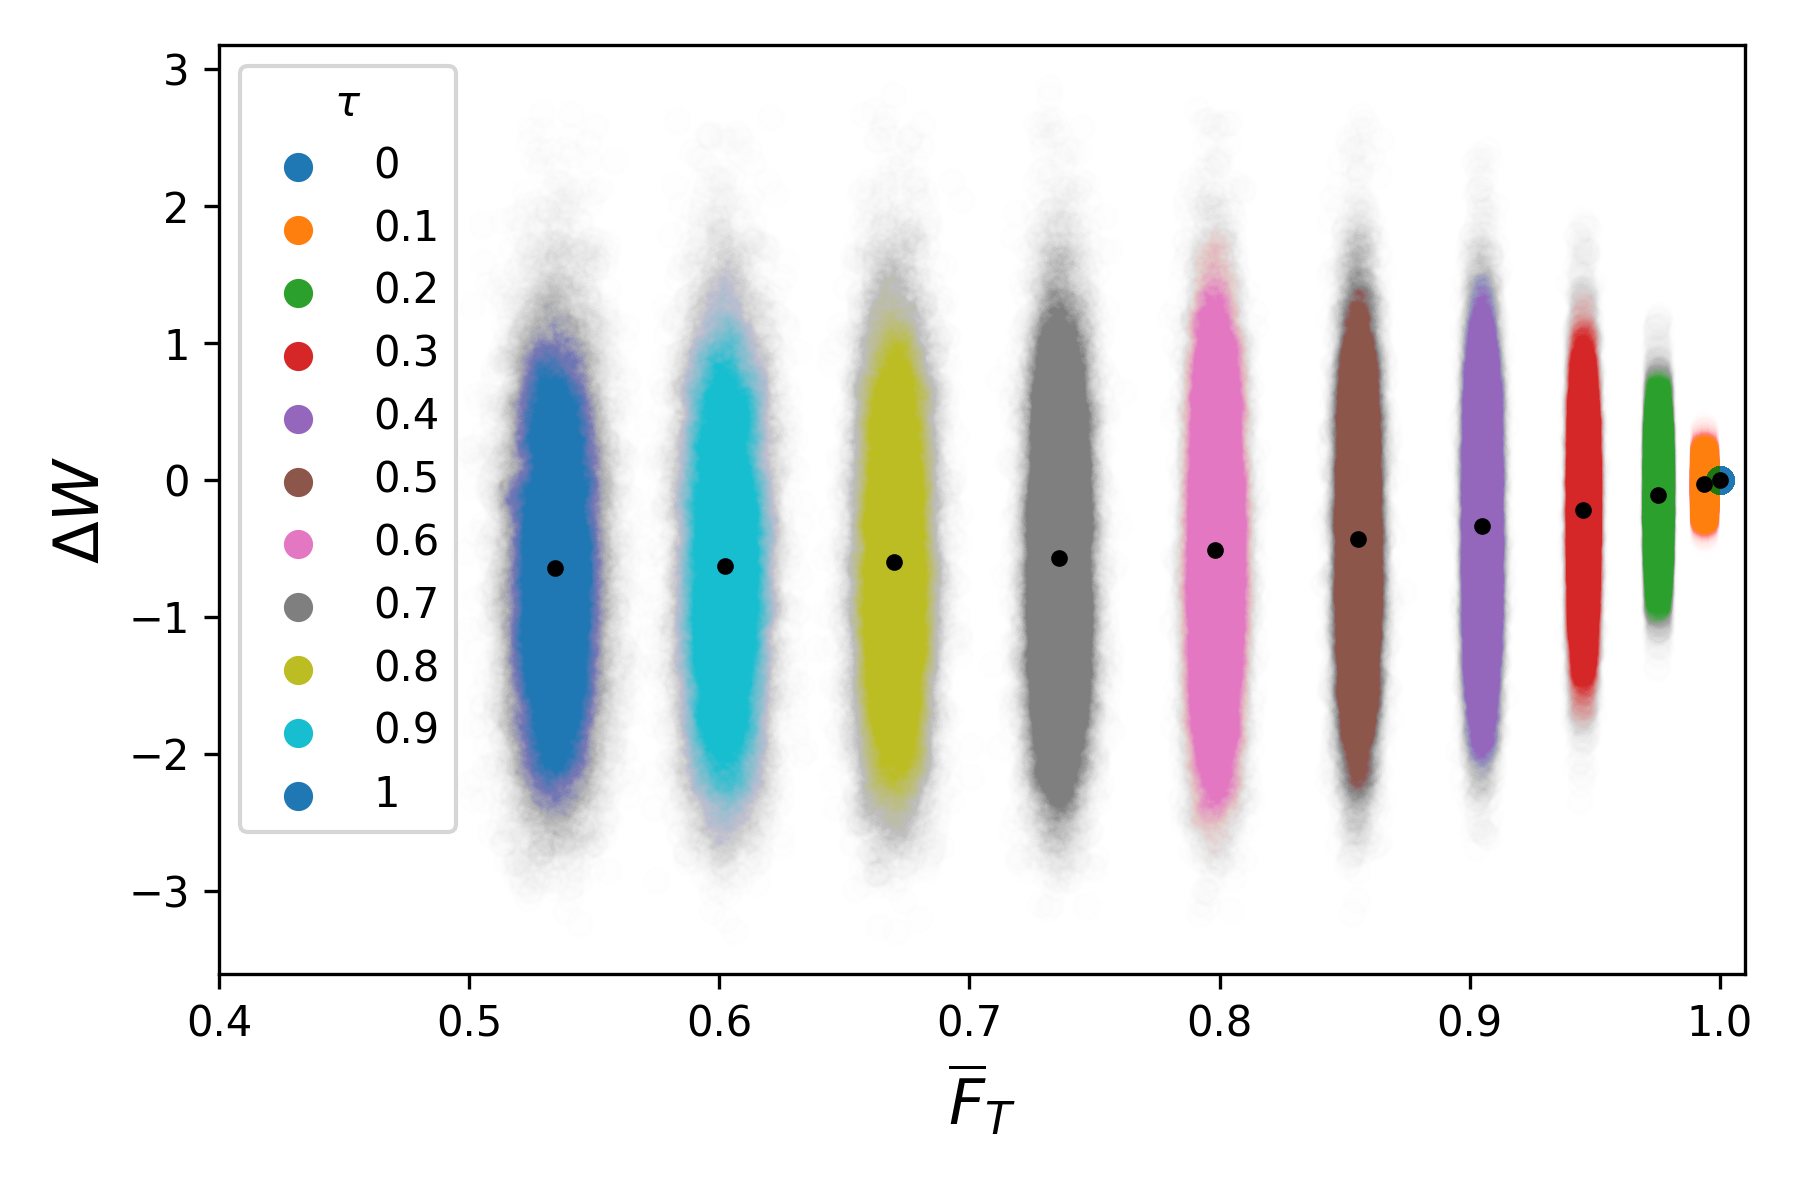
\includegraphics[width=\textwidth]{img/noisy_trans_bi_true_3}
		\subcaption{Noisy transducer sequence, $\Delta \mathrm{T} = 5$}
	\end{subfigure}
	\begin{subfigure}{0.4\textwidth}
		\centering
%		Hier kommt noch ein Bild
		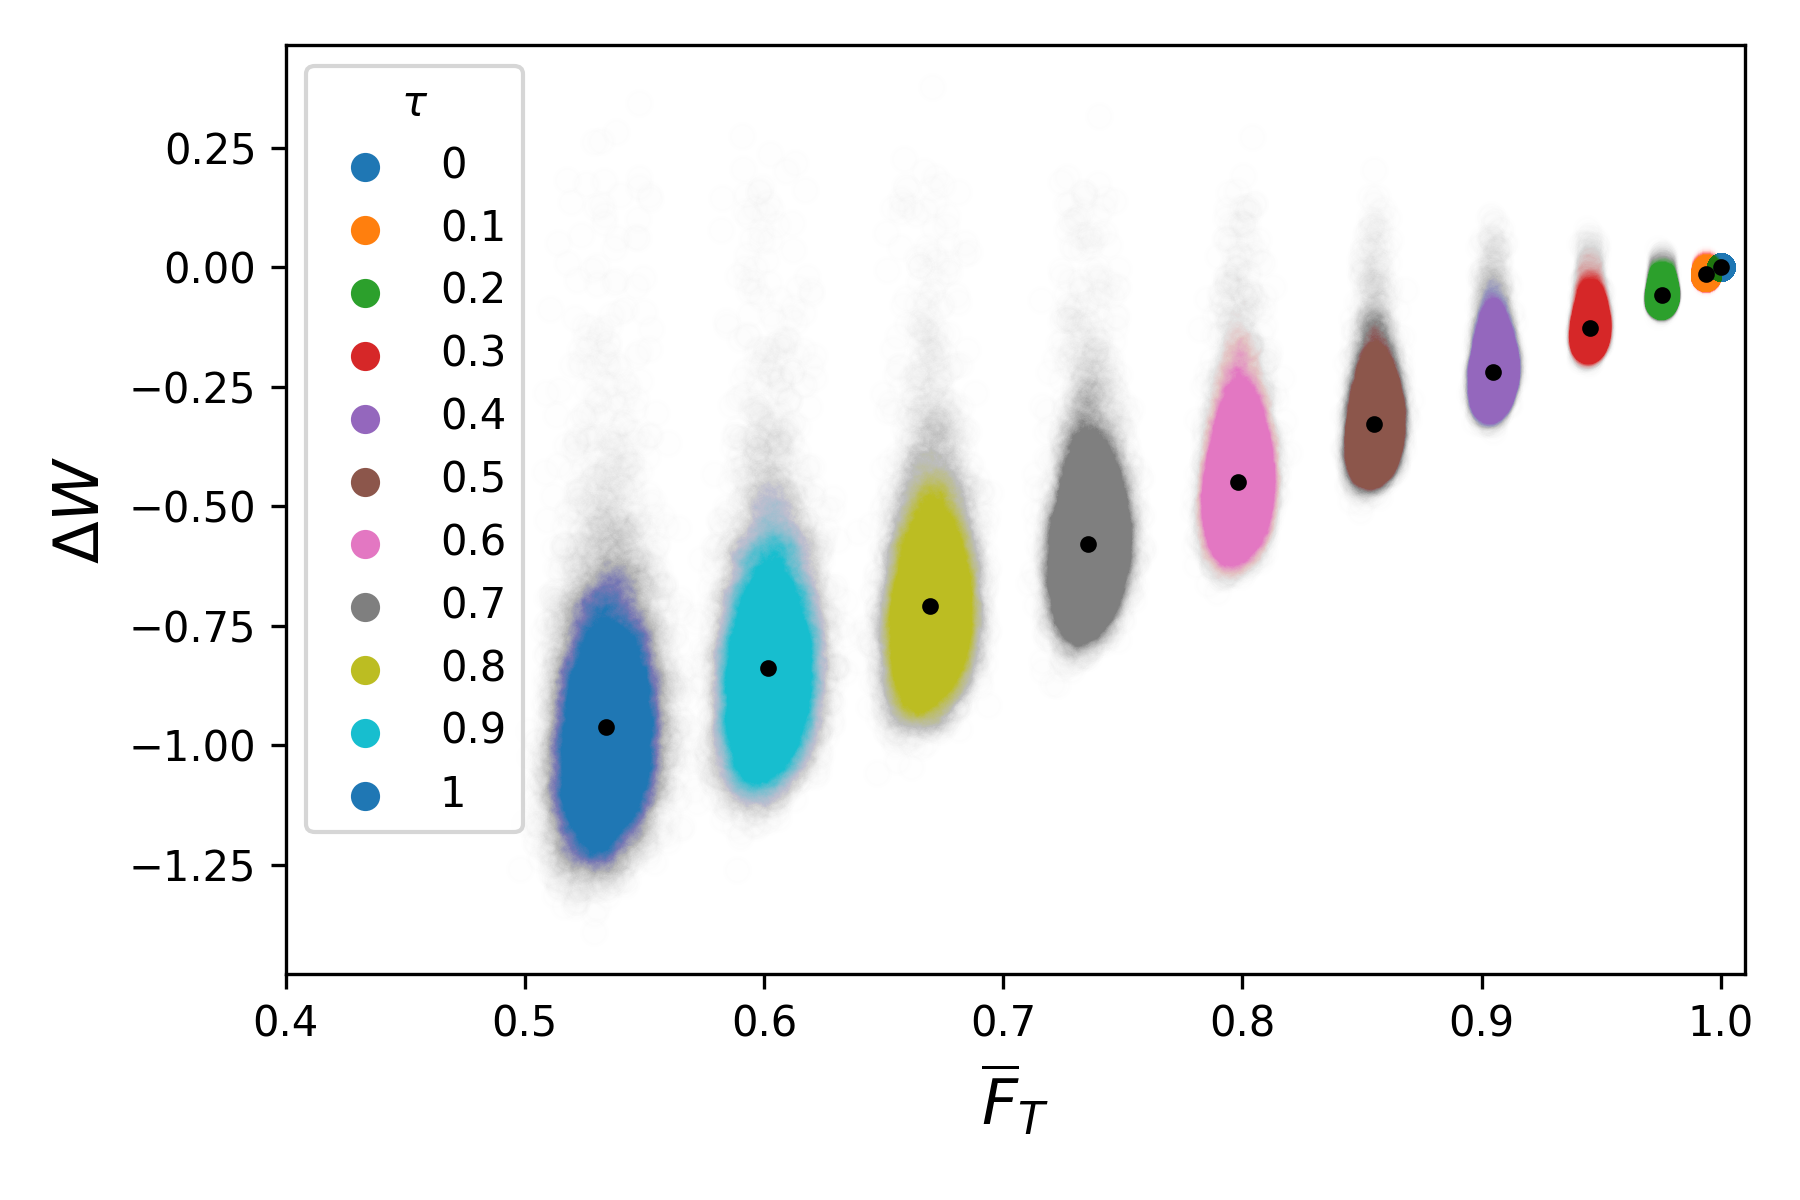
\includegraphics[width=\textwidth]{img/noisy_trans_dt_1}
		\subcaption{Noisy transducer sequence, $\Delta \mathrm{T} = 1$}
	\end{subfigure}
	\caption{We plot the difference $\Delta W = \overline{W}_{noise} - W_{pred}$ of each element of the test set for the bidirectional LSTM. $W_{pred}$ is the work output following the model prediction. \textbf{(a), (b)}: we create 100 noisy drive sequences and calculate the average $\overline{W}_{noise}$ of their work output following the predicted transducer protocol. \textbf{(c), (d)}: we create 100 noisy transducer sequences and calculate the average of their work output with a given drive sequence from the test set. In both plots, the black dots indicate the average fidelities and $\Delta W$ for a given $\tau$.}
	\label{noisedt5}
\end{figure}